\documentclass[12pt,answers]{exam}

\usepackage{amsmath,amsfonts,amssymb,mathtools,physics,commath}
\usepackage{todonotes}
\usepackage{float}
\usepackage{multicol}

\newcommand{\inv}{^{-1}}

\pagestyle{headandfoot}
\firstpageheadrule
\runningheadrule
\firstpageheader{Math 221}{Exam 1|Solutions, Page \thepage\ of \numpages}{February 5, 2019}
\runningheader{Math 221}{Exam 1|Solutions, Page \thepage\ of \numpages}{February 5, 2019}
\runningfooter{}{}{}

\begin{document}
% \maketitle
\begin{questions}
	\question
	Evaluate the following integrals.
	\begin{parts}
		\part[10]
		$\displaystyle \int \frac{e^x}{(1+e^x)^3} \dif x$
		\begin{solution}
			Let $u = e^x$, so $\dif u = e^x \dif x$.
			Then
			\begin{align*}
				\frac{e^x}{(1+e^x)^3} \dif x
				= \int u^{-3} \dif u 
				= \frac{u^{-2}}{-2}
				= \boxed{-\frac12(1+e^x)^{-2} + C}
			\end{align*}
		\end{solution}
		\part[10]
		$\displaystyle \int x \sqrt{x-1} \dif x$
		\begin{solution}
			Letting $u = x - 1$, so $\dif u = \dif x$ and $u+1 = x$
			Then
			\begin{align*}
				\int x \sqrt{x-1} \dif x
				 & = \int (u+1)\sqrt{u} \dif u \\
				 & = \int u^{3/2} + u^{1/2} \dif u \\
				 & = \frac25 u^{5/2} + \frac32 u^{3/2} \\
				 & = \boxed{\frac25(x-1)^{5/2} + \frac32 (x-1)^{3/2} + C}
			\end{align*}
		\end{solution}
	\end{parts}

\newpage
\question
Evaluate the following integrals.
\begin{parts}
	\part[10]
	$\displaystyle \int x^2 \ln(x) \dif x$
	\begin{solution}
		IBP:
		\[
			\begin{array}{ccc}
				  & D            & I              \\
				+ & \ln x        & x^2            \\
				- & \dfrac{1}{x} & \dfrac{x^3}{3}
			\end{array}
		\]
		so
		\begin{align*}
			\int x^2 \ln(x) \dif x
			 & = \frac{x^3}{3} \ln x - \int \frac13 x^2 \dif x  \\
			 & = \boxed{\frac{x^3}{3} \ln x - \frac 19 x^3 + C}
		\end{align*}
	\end{solution}
	\part[10]
	$\displaystyle \int \tan\inv x \dif x$, where $\tan\inv x = \arctan x$.
	\begin{solution}
		IBP:
		\[
			\begin{array}{ccc}
				  & D                & I \\
				+ & \tan\inv x       & 1 \\
				- & \dfrac{1}{x^2+1} & x
			\end{array}
		\]
		so
		\begin{align*}
			\int \tan\inv x \dif x
			 & = x \tan\inv x - \int \frac{x}{x^2+1} \dif x \\ 
			 & = \boxed{x \tan\inv x - \frac12 \ln(x^2+1) + C}
		\end{align*}
	\end{solution}
\end{parts}

\newpage
\question
Evaluate the following integrals.
\begin{parts}
	\part[10]
	$\displaystyle \int_0^1 \dfrac{\dif x}{\sqrt{4-x^2}}$
	\begin{solution}
		Using the general formula $\displaystyle \int \frac{\dif x}{\sqrt a^2-x^2} = \sin[-1](\frac xa) + C$ on the cover page:
		\begin{align*}
			\int_0^1 \dfrac{\dif x}{\sqrt{4-x^2}}
			 & = \eval{\sin[-1](\frac x2)}_0^1     \\
			 & = \sin[-1](\frac 12) - \sin[-1](0)  \\
			 & = \frac\pi6 - 0 = \boxed{\frac\pi6}
		\end{align*}
	\end{solution}
	\part[10]
	$\displaystyle \int \frac{\dif x}{\sqrt{1+x^2}}$
	\begin{solution}
		Using trig sub $x = \tan \theta$, so $\dif x = \sec^2 \theta \dif \theta$,
		\begin{multicols}{2}
			\begin{align*}
				\int \frac{\dif x}{\sqrt{1+x^2}}
				 & = \int \frac{\sec^2 \theta \dif \theta}{\sqrt{1+\tan^2 \theta}} \\
				 & = \int \frac{\sec^2 \theta \dif \theta}{\sqrt{\sec^2 \theta}}   \\
				 & = \int \sec \theta \dif \theta                                  \\
				 & = \ln \abs{\sec \theta + \tan\theta}                            \\
				 & = \boxed{\ln\abs{\sqrt{x^2+1} + x} + C}
			\end{align*}
			\begin{figure}[H]
				\centering
				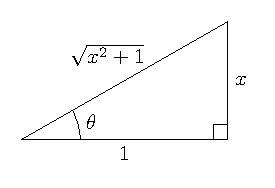
\includegraphics{graphics/2019-spring-exam1-3b.pdf}
			\end{figure}
		\end{multicols}
	\end{solution}
\end{parts}

\newpage
\question Evaluate the following integrals.
\begin{parts}
	\part[10] $\displaystyle \int \sin[3](x) \cos[8](x) \dif x$
	\begin{solution}
		\begin{align*}
\sin[3](x) \cos[8](x) \dif x
&= \int \sin x \underbracket{(1-\cos[2](x))}_{=\sin^2(x)} \cos[8](x) \dif x \\ 
&= - \int (1-u^2)u^8 \dif u \qquad (u = \cos x; \dif u = -\sin x \dif x)\\ 
&= -\int(u^8 - u^{10}) \dif u \\ 
&= - \frac19 u^9 + \frac{1}{11} u^{11} \\ 
&= \boxed{-\frac19 \cos[9](x) + \frac{1}{11} \cos[11](x) + C}
		\end{align*}
	\end{solution}
	\part[10] $\displaystyle \int \tan[4](x) \dif x$
	\begin{solution}
		Using reduction formula on cover page:
		\begin{align*}
			\int \tan[4](x) \dif x 
			= \frac{\tan[3](x)}{3} - \int \tan[2](x) \dif x \\ 
			= \frac{\tan[3](x)}{3} - \left(\tan x - \int 1 \dif x\right) \\ 
			= \boxed{\frac{\tan[3](x)}{3} - \tan x + x + C}
		\end{align*}
	\end{solution}
\end{parts}

\newpage
\question[10]
An object moves along a straight line with velocity function $v(t) = t e^{-t}$, in meters per second. Determine its change in position over the time interval $t = 0$ to $t = 4$ seconds.
\begin{solution}
	The object's displacement is given by the integral $\displaystyle \int_0^4 t e^{-t} \dif t$.
	Evaluating this uses IBP:
	\[
		\begin{array}{ccc}
			  & D & I       \\
			+ & t & e^{-t}  \\
			- & 1 & -e^{-t} \\
			+ & 0 & e^{-t}
		\end{array}
	\]
	Thus
	\begin{align*}
		\int_0^4 t e^{-t} \dif t
		 & = \eval{-te^{-t} - e^{-t}}_0^4 \\
		 & = -4 e^{-4} - e^{-4} - (0-1)
		= \boxed{-5e^{-4} + 1}
	\end{align*}
\end{solution}

% \newpage
\question[10]
Find a function $f(t)$ such that $f'(t) = s \tan(s^2) - \sec^2(s)$.
\begin{solution}
	\begin{align*}
		\int \left( s \tan(s^2) - \sec^2(s) \right)\dif t
		= \boxed{-\frac12 \ln\abs{\cos(s^2)} - \tan(s) + C}
	\end{align*}
	(Integrating the first term involves the $u$-sub $u = s^2$.)
\end{solution}
\end{questions}
\end{document}
